\chapter{Video}
\begin{multicols}{2}
ZX Spectrum Next video splits the display types into four categories
(layer 1 (ULA/Timex/LoRes), layer 2, layer 3 (tilemap) and sprites)
which have their own sets of controls for colour palettes, clipping,
and scrolling. Some aspects of ULA and tilemap are tied together, but
all the rest operate in a largely independent manner using a layering
system. The ULA category has a number of separate video modes that it
can use. One of these (LoRes) is incompatible with using tilemaps.
\section{General Features}
There are a number of control features for the various video modes
that are done in a unified fashion. These features are layering and
transparency, palettes, scrolling, and clipping. 

\subsection{Video Layering and Transparency}
Video is rendered as three layers which are referred to as ULA (which
includes the tilemap), layer 2, and sprites.  The ordering of the
layers is controlled by Next port \$15 (21) bits 4-2:

\begin{table}[h]\centering
  \caption{Video Layering}
  \csvautotabular{video/videolayering.csv}
\end{table}

\index{transparency}
Transparency for Layer 2, ULA, LoRes, and 1-bit Tilemaps are
controlled by Next register \$14 (20) and defaults to \$E3. Sprites
and 4-bit Tilemaps have their own registers (\$4B and \$4C
respectively) for setting their transparency index (not colour). This
colour ignores the state of the least significant blue bit, so \$E3
equates to both \$1C6 and \$1C7. For Sprites and Tilemaps transparency
is determined by colour index. For Sprites this is controlled by
register \$4B (with only the least significant 4-bits being relevant
for 16-colour Sprites). For Tilemaps, the transparency index is set by
register \$4C. If all layers are transparent, the transparency
fallback colour is displayed. This is set by register \$4A.

(R/W) \$14 (20) $\Rightarrow$ Global Transparency Colour
\begin{itemize}
\item bits 7-0 = 8-bit transparency colour (soft reset = \$E3)
\end{itemize}

(R/W) \$4A (74) $\Rightarrow$ Fallback colour
\begin{itemize}
\item bits 7-0 = 8-bit colour used if all layers are transparent (soft
  reset = 0)
\end{itemize}

(R/W) \$4B (75) $\Rightarrow$ Sprite transparency index
\begin{itemize}
\item bits 7-0 = Sprite colour index treated as transparent (soft
  reset = \$E3)
\item[] For 4-bit sprites only the bottom 4-bits are used
\end{itemize}

(R/W) \$4C (74) $\Rightarrow$ Tilemap transparency index
\begin{itemize}
\item bits 7-4 = Reserved, must be 0
\item bits 3-0 = Tilemap colour index treated as transparent (soft
  reset \$f)
\end{itemize}

\subsection{Palette}
\index{palette}
\paragraph{Next Colour Palettes}
Each video mode group has a pair of palettes assigned to it a primary
and an alternate palette. Each palette entry is actually a 9-bit value
(RRRGGGBBB) and can be set by selecting a palette using nextreg \$43
(palette control), the entry using nextreg \$40 (palette index), then
writing the value into nextreg \$44 (palette value, 9-bit) using pairs
of consecutive writes for each palette value or nextreg \$41 (palette
value, 8-bit). Once a palette index has been selected writes
automatically increment the palette index number so it is possible to
efficiently write the values for a collection of palette entries.

(R/W) \$40 (64) $\Rightarrow$ Palette Index
\begin{itemize}
\item bits 7-0 = Select the palette index to change the associated
  colour. (soft reset = 0)
\item[] For the ULA only, INKs are mapped to indices 0-7, Bright INKS
  to indices 8-15, PAPERs to indices 16-23 and Bright PAPERs to
  indices 24-31.  In ULANext mode, INKs come from a subset of indices
  0-127 and PAPERs come from a subset of indices 128-255.  The number
  of active indices depends on the number of attribute bits assigned
  to INK and PAPER out of the attribute byte.  In ULA+ mode, the top
  64 entries hold the ula+ palette.  The ULA always takes border
  colour from paper for standard ULA and ULAnext.
\end{itemize}

(R/W) \$41 (65) $\Rightarrow$ Palette Value (8 bit colour)
\begin{itemize}
\item bits 7-0 = Colour for the palette index selected by nextreg
  \$40.
\item[] The format is RRRGGGBB - the lower blue bit of the 9-bit
  colour will be the logical OR of blue bits 1 and 0 of this 8-bit
  value.
\item[] After the write, the palette index is auto-incremented to the
  next index if the auto-increment is enabled in nextreg \$43.  Reads
  do not auto-increment.  Any other bits associated with the index
  will be zeroed.
\end{itemize}

(R/W) \$43 (67) $\Rightarrow$ Palette Control
\begin{itemize}
\item bit 7 = Disable palette write auto-increment (soft reset = 0)
\item bits 6-4 = Select palette for reading or writing (soft reset =
  000)
  \begin{itemize}
  \item 000 = ULA first palette
  \item 100 = ULA second palette
  \item 001 = Layer 2 first palette
  \item 101 = Layer 2 second palette
  \item 010 = Sprites first palette 
  \item 110 = Sprites second palette
  \item 011 = Tilemap first palette
  \item 111 = Tilemap second palette
  \end{itemize}
\item bit 3 = Select Sprites palette (0 = first palette, 1 = second
  palette) (soft reset = 0)
\item bit 2 = Select Layer 2 palette (0 = first palette, 1 = second
  palette) (soft reset = 0)
\item bit 1 = Select ULA palette (0 = first palette, 1 = second
  palette) (soft reset = 0)
\item bit 0 = Enable ULANext mode (soft reset = 0)
\end{itemize}

(R/W) \$44 (68) $\Rightarrow$ Palette Value (9 bit colour)
\begin{itemize}
\item[] Two consecutive writes are needed to write the 9 bit colour
\item[] 1st write:
\item bits 7-0 = RRRGGGBB
\item[] 2nd write:
\item bits 7-1 = Reserved, must be 0
\item bit 0 = lsb B
\item[] If writing to an L2 palette
\item bit 7 = 1 for L2 priority colour, 0 for normal.
\item[] An L2 priority colour moves L2 above all layers.  If you need
  the same colour in both priority and normal modes, you will need to
  have two different entries with the same colour one with and one
  without priority.  If auto-increment is enabled in nextreg \$43, the
  palette index is auto-incremented after two consecutive writes
\item[] Reads only return the 2nd byte and do not auto-increment.
\item[] can also be read back from nextreg \$28
\end{itemize}

\subsection{Scrolling}
The ZX Spectrum Next has four sets of scrolling registers to
independently contol the display offsets of various video modes
(Layer2, ULA, Tilemap, and LoRes). When the video is offset, the
portion that is pushed off the screen (to the left and or top) then
becomes visible on the opposite side of the screen so that the video
offset values are effectively the coordinates of the origin in a
toroidal universe.

\subsection{Clipping}
The ZX Spectrum Next has four clipping registers create a window of
the layer that is visible. Clipping is managed by a set of four
successive writes to the clipping register applicable for the video
mode. If a section is masked off by clipping, it is as if the area
were the transparency colour and the video lyers behind it become
visible.

\section{Layer 1}
The Layer 1 consists of ZX Spectrum ULA video, Timex video modes, and
the Spectrum Next’s lores video modes all use 16k memory bank 5 or 7
with the data coming from some combination of addresses \$0000-\$17FF
(bitmap 1), \$1800-\$1AFF (attribute 1), \$2000-\$37FF (bitmap 2), and
\$3800-\$3AFF (attribute 2) within the selected bank.  Assuming
default memory mapping and the use of bank 5 this will be mapped as
some combination of memory \$4000-\$57FF, \$5800-\$5AFF,
\$6000-\$77FF, \$780-\$7AFF. All of the modes other than the lores
mode can either use the default ZX Spectrum colours, ULANext mode, or
an emulation of ULAplus. In the Spectrum and Timex modes all colours are
either Paper (foreground), paper (background), or border colours.

\subsection{Colour Attributes}
The ZX Spectrum Next has three major modes for colour attributes: the
ZX Spectrum attribute mapping, which is augmented by using the ZX
Spectrum Next's palette; ULANext, which allows the user to how many
foreground and how many background colous are to be selected by the
attribute bytes; and an emulation of ULAplus.

\paragraph{ULA Colour}
In ULA colour INKs are mapped to indices 0-7, Bright INKS to indices
8-15, PAPERs to indices 16-23 and Bright PAPERs to indices 24-31. This
is the default state for interpreting ULA palettes.

\begin{table}[h]\centering
  \caption{ULA Colour}
  \csvautotabular{video/flash.csv}
\end{table}

\paragraph{ULANext}
The ULANext modes use a varying number of bits from the attribute
byte to determine the ink colours as the palette index from the
appropriate bits (all others being zero) and the paper colours coming
from the indicated value+128 with palette format 255 being a special
case where all the bits determine the ink colour while the paper is
always palette index 128. The ULA always takes border colour from
paper. ULANext is enabled using bit 0 of nextreg \$43 (palette
control) and controlled with nextreg \$42 (ULA Next attribute byte
format)

\begin{table}[h]\centering
  \caption{ULANext}
  \csvautotabular{video/palfmt.csv}
\end{table}

\paragraph{ULAplus}
The ZX Next emulates ULAPlus using the last 64 (192-255) entries of
the ULA palette. ULAplus is controlled using two ports: \$BF3B (register
port) and \$FF3B (data port)

\subparagraph{I/O ports}
ULAplus is controlled by two ports.

\$BF3B is the register port (write only)

The byte output will be interpreted as follows:
\begin{itemize}
\item Bits 7-6: Select the register group. Two groups are currently available:
  \begin{itemize}
  \item 00=palette group\\
    When this group is selected, the sub-group determines the entry in the
    palette table (0-63).
  \item 01=mode group\\
    The sub-group is (optionally) used to mirror the video functionality
    of Timex port \$FF as follows:
  \end{itemize}
\item Bits 5-0: Select the register sub-group
\item[] Mode group
\item Bits 5-3: Sets the screen colour in hi-res mode.
  \begin{itemize}
  \item 000=Black on White
  \item 001=Blue on Yellow
  \item 010=Red on Cyan
  \item 011=Magenta on Green
  \item 100=Green on Magenta
  \item 101=Cyan on Red
  \item 110=Yellow on Blue
  \item 111=White on Black
  \end{itemize}
\item Bits 2-0: Screen mode.
  \begin{itemize}
  \item 000=screen 0 (bank 5)
  \item 001=screen 1 (bank 5)
  \item 010=hi-colour (bank 5)
  \item 100=screen 0 (bank 7)
  \item 101=screen 1 (bank 7)
  \item 110=hi-colour (bank 7)
  \item 110=hi-res (bank 5)
  \item 111=hi-res (bank 7)
  \end{itemize}
\end{itemize}

\$FF3B is the data port (read/write)

When the palette group is selected, the byte written will describe the
color.

When the mode group is selected, the byte output will be interpreted
as follows:
\begin{itemize}
\item Bit 0: ULAplus palette on (1) / off (0)
\item Bit 1: (optional) grayscale: on (1) / off (0) (same as turing
  the color off on the television)
\end{itemize}

Implementations that support the Timex video modes use the \$FF
register as the primary means to set the video mode, as per the Timex
machines. It is left to the individual implementations to determine if
reading the port returns the previous write or the floating bus.

\subparagraph{GRB palette entries}

G3R3B2 encoding\\
For a device using the GRB colour space the palette entry is
interpreted as follows
\begin{itemize}
\item Bits 7-5: Green intensity.
\item Bits 4-2: Red intensity.
\item Bits 1-0: Blue intensity.
\end{itemize}

This colour space uses a sub-set of 9-bit GRB. The missing lowest blue
bit is set to OR of the other two blue bits (Bb becomes 000 for 00,
and Bb1 for anything else). This gives access to a fixed half the
potential 512 colour palette. The reduces the jump in intensity in the
lower range in the earlier version of the specification. It also means
the standard palette can now be represented by the ULAplus palette.

\subparagraph{Grayscale palette entries}
In grayscale mode, each palette entry describes an intensity from zero
to 255. This can be achieved by simply removing the colour from the
output signal.

\subparagraph{Limitations}
Although in theory 64 colours can be displayed at once, in practice
this is usually not possible except when displaying colour bars,
because the four CLUTs are mutually exclusive; it is not possible to
mix colours from two CLUTs in the same cell. However, with software
palette cycling it is possible to display all 256 colours on screen at
once.

\subparagraph{Emulation}
The 64 colour mode lookup table is organized as 4 palettes of 16
colours.

Bits 7 and 6 of each Spectrum attribute byte (normally used for FLASH
and BRIGHT) will be used as an index value (0-3) to select one of the
four colour palettes.

Each colour palette has 16 entries (8 for INK, 8 for PAPER). Bits 0 to
2 (INK) and 3 to 5 (PAPER) of the attribute byte will be used as
indexes to retrieve colour data from the selected palette.

With the standard Spectrum display, the BORDER colour is the same as
the PAPER colour in the first CLUT. For example BORDER 0 would set the
border to the same colour as PAPER 0 (with the BRIGHT and FLASH bits
not set).

The complete index can be calculated as\\
ink\_colour = (FLASH * 2 + BRIGHT) * 16 + INK
paper\_colour = (FLASH * 2 + BRIGHT) * 16 + PAPER + 8

\subparagraph{Palette file format}
The palette format doubles as the BASIC patch loader. This enables you
to edit patches produced by other people.
\begin{verbatim}
; 64 colour palette file format (internal) - version 1.0
; copyright (c) 2009 Andrew Owen
;
; The palette file is stored as a BASIC program with embedded machine code

header:

db 0x00 ; program file
db 0x14, 0x01, "64colour" ; file name
dw 0x0097 ; data length
dw 0x0000 ; autostart line
dw 0x0097 ; program length

basic:

; 0 RANDOMIZE USR ((PEEK VAL "2
; 3635"+VAL "256"*PEEK VAL "23636"
; )+VAL "48"): LOAD "": REM

db 0x00, 0x00, 0x93, 0x00, 0xf9, 0xc0, 0x28, 0x28
db 0xbe, 0xb0, 0x22, 0x32, 0x33, 0x36, 0x33, 0x35
db 0x22, 0x2b, 0xb0, 0x22, 0x32, 0x35, 0x36, 0x22
db 0x2a, 0xbe, 0xb0, 0x22, 0x32, 0x33, 0x36, 0x33
db 0x36, 0x22, 0x29, 0x2b, 0xb0, 0x22, 0x34, 0x38
db 0x22, 0x29, 0x3a, 0xef, 0x22, 0x22, 0x3a, 0xea

start:

di ; disable interrupts
ld hl, 38 ; HL = length of code
add hl, bc ; BC = entry point (start) from BASIC
ld bc, 0xbf3b ; register select
ld a, 64 ; mode group
out (c), a ;
ld a, 1 ;
ld b, 0xff ; choose register port
out (c), a ; turn palette mode on
xor a ; first register

setreg:

ld b, 0xbf ; choose register port
out (c), a ; select register
ex af, af' ; save current register select
ld a, (hl) ; get data
ld b, 0xff ; choose data port
out (c), a ; set it
ex af, af' ; restore current register
inc hl ; advance pointer
inc a ; increase register
cp 64 ; are we nearly there yet?
jr nz, setreg ; repeat until all 64 have been done
ei ; enable interrupts
ret ; return

; this is where the actual data is stored. The following is an example palette.

registers:

db 0x00, 0x02, 0x18, 0x1b, 0xc0, 0xc3, 0xd8, 0xdb ; INK
db 0x00, 0x02, 0x18, 0x1b, 0xc0, 0xc3, 0xd8, 0xdb ; PAPER
db 0x00, 0x03, 0x1c, 0x1f, 0xe0, 0xe3, 0xfc, 0xff ; +BRIGHT
db 0x00, 0x03, 0x1c, 0x1f, 0xe0, 0xe3, 0xfc, 0xff ;
db 0xdb, 0xd8, 0xc3, 0xc0, 0x1b, 0x18, 0x02, 0x00 ; +FLASH
db 0xdb, 0xd8, 0xc3, 0xc0, 0x1b, 0x18, 0x02, 0x00 ;
db 0xff, 0xfc, 0xe3, 0xe0, 0x1f, 0x1c, 0x03, 0x00 ; +BRIGHT/
db 0xff, 0xfc, 0xe3, 0xe0, 0x1f, 0x1c, 0x03, 0x00 ; +FLASH

terminating_byte:

db 0x0d 
\end{verbatim}

\subsection{Layer 1 Scrolling}
Layer 1 has two sets of scrolling registers. One for the the legacy
modes (ZX Spectrum, Alternate Page, Timex Hi-Resoulution, and Timex
Hi-colour) and a second set for the two ZX Spextrum Next specific
LoRes modes.  All modes scroll as if they were $256\times192$ screens
located at global coordinates (32, 32) to (287, 223), The registers
for the legacy modes are \$26 and \$27 and the registers for the LoRes
modes are \$32 and \$33.

\register{R/W}{26}{ULA Horizontal Scroll Control}
\begin{itemize}
\item bits 7-0 = ULA X Offset (0-255) (0 on reset)
\end{itemize}


\register{R/W}{27}{ULA Vertical Scroll Control}
\begin{itemize}
\item bits 7-0 = ULA Y Offset (0-191) (0 on reset)
\end{itemize}


\register{R/W}{32}{Layer 1,0 (LoRes) Horizontal Scroll Control)}
\begin{itemize}
\item bits 7-0 = X Offset (0-255) (\$00 on reset)
\end{itemize}
Layer 1,0 (LoRes) scrolls in "half-pixels" at the same resolution and
smoothness as Layer 2.


\register{R/W}{33}{Layer 1,0 (LoRes) Vertical Scroll Control)}
\begin{itemize}
\item bits 7-0 = Y Offset (0-191) (\$00 on reset)
\end{itemize}
Layer 1,0 (LoRes) scrolls in "half-pixels" at the same resolution and
smoothness as Layer 2.



\subsection{Layer 1 Clipping}
All of the modes in the Layer 1 share a single clipping register,
\$1A. The clip index may alternately be set using register \$1C. This
is expecially useful for reading the current clipping coordinates as
reads on the clipping register do not change the index. Note that
clipping coordinates are based on a full display area for the mode of
$256\times192$ resolution even though not all modes have that
resolution.

\register{R/W}{1A}{Layer 0 (ULA/LoRes) Clip Window Definition}
\begin{itemize}
\item bits 7-0 = Coord. of the clip window
  \begin{itemize}
  \item[] 1st write = X1 position
  \item[] 2nd write = X2 position
  \item[] 3rd write = Y1 position
  \item[] 4rd write = Y2 position
  \end{itemize}
\end{itemize}
The values are 0,255,0,191 after a Reset\\
Reads do not advance the clip position


\register{R/W}{1C}{Clip Window Control}\\
Read
\begin{itemize}
\item bits 7-6 = Layer 3 Clip Index
\item bits 5-4 = Layer 0/1 Clip Index
\item bits 3-2 = Sprite clip index
\item bits 1-0 = Layer 2 Clip Index
\end{itemize}
Write
\begin{itemize}
\item bits 7-4 = Reserved, must be 0
\item bit 3 - reset Layer 3 clip index
\item bit 2 - reset Layer 0/1 clip index
\item bit 1 - reset sprite clip index.
\item bit 0 - reset Layer 2 clip index.
\end{itemize}



\subsection{ZX Spectrum Mode}

Timex mode 0

This is the default ULA mode and has its origins in the original ZX
Spectrum. It uses $256\times192$ pixels located at global coordinates
(32, 32) to (287, 223) with $8\times8$ colour attribute areas mapped
into a $32\times24$ grid. If Timex modes are not enabled, this and the
LoRes mode are the only ones available, so you would switch back to
this mode by writing 000xxxxx to Next register \$15 (21, the sprites
and layers register). If another Timex mode is enabled, then this is
mode 0 so you would write 0 to port \$ff to enable it. This is a
$256\times192$ video mode. The bitmap 1 area is used for selection
between ink and paper colours with one bit per pixel and the attribute
1 area for colour attributes.

The easiest way to visualize the mapping of this mode is to think of
the $256\times192$ area as being divided into a $32\times24$ grid of
$8\times8$ characters.  IF we consider X and Y as the position in the
grid and R to the the row within the character.  For ink/paper
selection, 0=paper, 1=ink and the entries are stored left to right as
lsb to msb within the bye.  The address for a pixel value is:
$0R_4R_3Y_2Y_1Y_0R_2R_1R_0C_4C_3C_2C_1C_0$. Each $8\times8$ cell has
its own colour attribute where the address for an attribute cell is
$0110R_4R_3R_2R_1R_0C_4C_3C_2C_1C_0$ in other words mapped lineally
column-wise starting at the beginning of the attribute 1 area.

Code:
\begin{verbatim}
  ;; from any other Timex mode:
  ld a,$00
  ld c,$ff
  out (c),a

  ;; from LoRes mode:
  ld bc,$243B ; next register select port
  ld a,$15
  out (c),a
  ld bc,$253B ; next register r/w port
  in a,(c)
  and $7f
  out (c),a
\end{verbatim}

\subsection{Alternate Page Mode}

Timex mode 1

This mode is the same as ZX Spectrum mode except it is at an alternate
addresses. Alternate page mode is selected by enabling Timex modes by
writing 00xxxx1xx to Next register \$08 (8, Peripheral 3 setting) then
writing 1 to the Timex ULA port (\$ff).  It is identical to ZX
Spectrum mode except the pixel are mapped to the bitmap 2 area giving
use pixel addresses of $1R_4R_3Y_2Y_1Y_0R_2R_1R_0C_4C_3C_2C_1C_0$ and
the attributes to the attribute 2 area with addresses of
$1110R_4R_3R_2R_1R_0C_4C_3C_2C_1C_0$.

Code:

\begin{verbatim}
;; disable LoRes mode:
ld bc,$243B ; next register select port
ld a,$15
out (c),a
ld bc,$253B ; next register r/w port
in a,(c)
and $7f
out (c),a
;; set Timex mode
ld bc,$243B ; next register select port
ld a,$08
out (c),a
ld bc,$253B ; next register r/w port
in a,(c)
or $04
out (c),a
;; set alternate page mode
ld c,$ff
ld a,$01
out (c),a
\end{verbatim}

\subsection{Timex Hi-Colour Mode}

Timex mode 2

This mode is a $256\times192$ video mode located at global coordinates
(32, 32) to (287, 223) with $8\times1$ colour attribute mapping on a
$32\times192$ grid. It is selected by writing 2 to the Timex ULA port
(\$ff).  Pixel mapping in this mode is the same as in ZX Spectrum mode
using the bitmap 1 area based on
$0R_4R_3Y_2Y_1Y_0R_2R_1R_0C_4C_3C_2C_1C_0$.  The colour attributes use
the bitmap 2 area with $8\times1$ colour attribute areas corresponding
to the addresses $1R_4R_3Y_2Y_1Y_0R_2R_1R_0C_4C_3C_2C_1C_0$.

Code:
\begin{verbatim}
;; disable LoRes mode:
ld bc,$243B ; next register select port
ld a,$15
out (c),a
ld bc,$253B ; next register r/w port
in a,(c)
and $7f
out (c),a
;; set Timex mode
ld bc,$243B ; next register select port
ld a,$08
out (c),a
ld bc,$253B ; next register r/w port
in a,(c)
or $04
out (c),a
;; set hi-colour mode
ld c,$ff
ld a,$02
out (c),a
\end{verbatim}

\subsection{Timex Hi-Resolution Mode}

Timex mode 6

This is a monochrome $512\times192$ video mode located at global
coordinates (32, 32) to (287, 223) with each pixel being half
width. It is selected by writing to the Timex ULA port (\$ff with
values that also select which two colours (or colour entries in
ULANext mode) you use.

\begin{table}[h]\centering
  \caption{Hi-Resolution Colours}
  \csvautotabular{video/hires.csv}
\end{table}
  
Pixels are mapped into both the bitmap 1 and bitmap 2 areas where
8-pixel wide character columns alternate between the two bitmap areas.
The pixels within a byte being rendered left to right lsb to msb as in
other Spectrum video modes.  The addresses for each row within a
character are based on a $64\times32$ grid of $8\times8$ characters
which using a $64\times24$ R, C, and Y scheme gives us addresses of
the form $C_0R_4R_3Y_2Y_1Y_0R_2R_1R_0C_5C_4C_3C_2C_1$.

Code:
\begin{verbatim}
;; disable LoRes mode:
ld bc,$243B ; next register select port
ld a,$15
out (c),a
ld bc,$253B ; next register r/w port
in a,(c)
and $7f
out (c),a
;; set Timex mode
ld bc,$243B ; next register select port
ld a,$08
out (c),a
ld bc,$253B ; next register r/w port
in a,(c)
or $04
out (c),a
;; set hi-res mode, black on white
ld c,$ff
ld a,$06
out (c),a
\end{verbatim}

\subsection{Lo-Resolution Mode}
This is a Spectrum Next specific video mode with a resolution of
$128\times96$ located at global coordinates (32, 32) to (287, 223)
with each pixel being double height and double width replacing the old
Radistan mode.  It can either allow for 16 colours, in which case it
uses either the bitmap 1 area or the bitmap 2 area, or 256 colours
using both bitmap 1 and bitmap 2. The colour of each pixel can be
selected independently with data ordered linearly in a row major
fashion. In the case of 16 colour mode, the nybbles describing the
colours are X major (MSN LSN). Scrolling is by half pixels and uses
different registers (\$32 and \$33) from the rest of the ULA group
modes. LoRes mode is enabled by writing $100xxxxx$ to Next register
\$15 (the sprites and layers register) with Next register \$6A used to
decide whether it is 16 or 256 colours.

\register{R/W}{15}{Sprite and Layer System Setup}
\begin{itemize}
\item bit 7 = LoRes mode (0 on reset)
\item bit 6 = Sprite priority (1 = sprite 0 on top, 0 = sprite 127 on
  top) (0 on reset)
\item bit 5 = Enable sprite clipping in over border mode (0 on reset)
\item bits 4-2 = set layers priorities (000 on reset)
  \begin{itemize}
  \item 000 - S L U
  \item 001 - L S U
  \item 010 - S U L
  \item 011 - L U S
  \item 100 - U S L
  \item 101 - U L S
  \item 110 - S(U+L) ULA and Layer 2 combined, colours clamped to 7
  \item 111 - S(U+L-5) ULA and Layer 2 combined, colours clamped to [0,7]
  \end{itemize}
\item bit 1 = Enable Sprites Over border (0 on reset)
\item bit 0 = Enable Sprites (0 on reset)
\end{itemize}


\register{R/W}{32}{Layer 1,0 (LoRes) Horizontal Scroll Control)}
\begin{itemize}
\item bits 7-0 = X Offset (0-255) (\$00 on reset)
\end{itemize}
Layer 1,0 (LoRes) scrolls in "half-pixels" at the same resolution and
smoothness as Layer 2.


\register{R/W}{33}{Layer 1,0 (LoRes) Vertical Scroll Control)}
\begin{itemize}
\item bits 7-0 = Y Offset (0-191) (\$00 on reset)
\end{itemize}
Layer 1,0 (LoRes) scrolls in "half-pixels" at the same resolution and
smoothness as Layer 2.


\register{R/W}{6A}{Layer 1,0 (LoRes) Control}
\begin{itemize}
\item bits 7-6 = reserved, must be 0
\item bit 5 = Enable Radistan (16-colour) (0 on reset)
\item bit 4 = Radistan DFILE switch (xor with bit 0 of port \$ff) (0
  on reset)
\item bits 3-0 = Radistsan palette offset (0 on reset)
\item bits 1-0 = ULAplus palette offset (0 on reset)
\end{itemize}



Code: 256 colour
\begin{verbatim}
;; enable LoRes mode:
nextreg $15,$80
;; 256-colour mode
ld bc,$243B ; next register select port
ld a,$6A
out (c),a
ld bc,$253B ; next register r/w port
in a,(c)
and $EF ; lores radistan control
out (c),a
\end{verbatim}

Code: 16 colour
\begin{verbatim}
;; enable LoRes mode:
nextreg $15,$80
;; 16-colour mode
nextreg $6A,$10
\end{verbatim}

\section{Layer 2}
Layer 2 is a linearly mapped, row-wise, upper left to lower right,
bit-map graphics area.  It supports modes with $256\times192\times256$
resolution at global coordinates (32, 32) to (287, 223),
$320\times256\times256$ resolution at global coordinates (0, 0) to
(318, 255), and $640\times256\times16$ resolution at global
coordinates (0, 0) to (319, 255) with half width pixels. It can be
mapped starting at any 16k memory blocks. The $256\times192\times256$
mode requires 3 consecutive blocks (48k) while the others use 5
consecutive blocks (80k).

\subsection{Configuration}
Layer 2 is enabled using port \$123B or register \$69. The mode is
selected using register \$70. How layer 2 memory is overlaid on main
memory is controled by port \$123B and register \$70. The location in
memory is controlled by register \$12 with a shadow area pointed to by
register \$13 for double buffering. Finally port \$123B is used to
select either the main RAM area or the shadow RAM area for rendering
the layer.

\port{123B}{Layer 2}\\
Bit 4 = 0
\begin{itemize}
\item[] bits 7-6 = Video RAM bank select
  \begin{itemize}
  \item[] 00 = first 16k
  \item[] 01 = second 16k
  \item[] 10 = third 16k
  \item[] 11 = first 48k
  \end{itemize}
\item[] bit 5 = Reserved, must be 0
\item[] bit 4 = 0
\item[] bit 3 = Shadow layer 2 select
\item[] bit 2 = Enable layer 2 read paging
\item[] bit 1 = Layer 2 visible (mirrored in register \$69)
\item[] bit 0 = Enable layer 2 write paging
\end{itemize}
Bit 4 = 1
\begin{itemize}
\item[] bits 7-5 = Reserved, must be 0
\item[] bit 4 = 1
\item[] bit 3 = Reserved, must be 0
\item[] bit 2-0 = 16k bank relative offset
\end{itemize}


\register{R/W}{12}{Layer 2 Active RAM bank}
\begin{itemize}
\item bits 7-6 = Reserved, must be 0
\item bits 5-0 = RAM bank (point to bank 8 after a Reset, NextZXOS
  modifies to 9)
\end{itemize}


\register{R/W}{13}{Layer 2 Shadow RAM bank}
\begin{itemize}
\item bits 7-6 = Reserved, must be 0
\item bits 5-0 = RAM bank (point to bank 11 after a Reset, NextZXOS
  modifies to 12)
\end{itemize}


\register{R/W}{69}{Display Control 1}
\begin{itemize}
\item bit 7 = Layer 2 Enable (Port \$123B bit 1 alias)
\item bit 6 = ULA Shadow display enable (Port \$7FFD bit 3 alias)
\item bits 5-0 = Timex alias (Port \$FF alias)
\end{itemize}


\register{R/W}{70}{Layer 2 Control}
\begin{itemize}
\item bits 7-6 = Reserved, must be 0
\item bits 5-4 = Resolution (00 on soft reset)
  \begin{itemize}
  \item 00 = $256\times192\times256$
  \item 01 = $320\times256\times256$
  \item 10 = $640\times256\times16$
  \item 11 = Do not use
  \end{itemize}
\item bits 3-0 = Palette offset (\$0 on soft reset)
\end{itemize}


\sinset
Code:
\paragraph{Layer 2 $256\times192$, Write only overlaid on ROM}
\begin{verbatim}
p_layer2: defl $123b
start:
  ld bc,p_layer2
  ld a,$03       ; enable, wo, 1st 16k
  out (c),a
  call wrtpage
  ld bc,p_layer2
  ld a,$43       ; enable, wo, 2nd 16k
  out (c),a
  call wrtpage
  ld bc,p_layer2
  ld a,$83       ; enable, wo, 3rd 16k
  out (c),a
  call wrtpage
  ret
wrtpage:  
  ld hl,$0000
  ld bc,$0040    ; 40*256 writes
loop:
  ld (hl),b
  inc hl
  djnz loop
  dec c
  jr nz,loop
\end{verbatim}
\paragraph{Layer 2 $256\times192$ resolution}
\begin{verbatim}
r_mmu_7:  defl $57
r_disp1:  defl $69
r_layer2: defl $70
start:
  nextreg r_disp1,$80  ; enable layer 2
  nextreg r_layer2,$00 ; 256x192x256
  ld a,$12             ; page 18=bank 9
loop1:
  nextreg r_mmu_7,a    ; map page into slot 7
  ld bc,$0020          ; 20*256 = 8k
  ld hl,$E000          ; address of slot 7
loop2:
  ld (hl),b
  inc hl
  djnz loop2
  dec c
  jp NZ,loop2
  inc a
  cp $18               ; stop at page 24
  jp NZ,loop1
\end{verbatim}
\paragraph{Layer 2 $320\times256$ resolution}
\begin{verbatim}
r_mmu_7:  defl $57
r_disp1:  defl $69
r_layer2: defl $70
start:
  nextreg r_disp1,$80  ; enable layer 2
  nextreg r_layer2,$10 ; 320x256x256
  ld a,$12             ; page 18=bank 9
loop1:
  nextreg r_mmu_7,a    ; map page into slot 7
  ld bc,$0020          ; 20*256 = 8k
  ld hl,$E000          ; start of slot 7
loop2:
  ld (hl),b
  inc hl
  djnz loop2
  dec c
  jp NZ,loop2
  inc a
  cp $1C               ; stop at page 28
  jp NZ,loop1
\end{verbatim}
\paragraph{Layer 2 $640\times256$ resolution}
\begin{verbatim}
r_mmu_7:  defl $57
r_disp1:  defl $69
r_layer2:  defl $70
start:
  nextreg r_disp1, $80   ; enable layer 2
  nextreg r_layer2, $20  ; 640x256x16
  ld a, $12    ; page 18=bank 9
loop1:
  nextreg r_mmu_7, a  ; map page into slot 7
  ld bc, $0020    ; 20*256 = 8k
  ld hl, $E000    ; start address for slot 7
loop2:
  ld (hl), b
  inc hl
  djnz loop2
  dec c
  jp NZ, loop2
  inc a
  cp $1C      ; stop at page 28
  jp NZ, loop1
\end{verbatim}
\einset

\subsection{Scrolling}
Scrolling Layer 2 is controlled by registers \$16 and \$17. (Is there
a third scrolling register for layer 2?)

\register{R/W}{16}{Layer 2 Horizontal Scroll Control}
\begin{itemize}
\item bits 7-0 = X Offset (0-255)(0 on reset)
\end{itemize}


\register{R/W}{17}{Layer 2 Vertical Scroll Control}
\begin{itemize}
\item bits 7-0 = Y Offset (0-191)(0 on reset)
\end{itemize}



\subsection{Clipping}
The Clip area for is based on the local coordinate system for the mode
in question and is set using register \$18 with the option of
selection which write in active using register \$1C.

\register{R/W}{18}{Layer 2 Clip Window Definition}
\begin{itemize}
\item bits 7-0 = Coords of the clip window
  \begin{itemize}
  \item[] 1st write - X1 position
  \item[] 2nd write - X2 position
  \item[] 3rd write - Y1 position
  \item[] 4rd write - Y2 position
  \end{itemize}
\end{itemize}
Reads do not advance the clip position\\
The values are 0,255,0,191 after a Reset


\register{R/W}{1C}{Clip Window Control}\\
Read
\begin{itemize}
\item bits 7-6 = Layer 3 Clip Index
\item bits 5-4 = Layer 0/1 Clip Index
\item bits 3-2 = Sprite clip index
\item bits 1-0 = Layer 2 Clip Index
\end{itemize}
Write
\begin{itemize}
\item bits 7-4 = Reserved, must be 0
\item bit 3 - reset Layer 3 clip index
\item bit 2 - reset Layer 0/1 clip index
\item bit 1 - reset sprite clip index.
\item bit 0 - reset Layer 2 clip index.
\end{itemize}



\section{Layer 3 (Tilemap) Mode}

Started with documentation by Phoebus Dokos, February 25,
2019. Partially rewritten for clarity and to add core 3.00.00
features.

\subsection{General Description}
The tilemap is a hardware character oriented display. It uses a set of
user defined 4-bit, 16-colour, or 1-bit, 2-colour $8\times8$
tiles. The tiles can be dispplayed in two resolutions: $40\times32$
tiles ($320\times256$ pixels) and $80\times32$ tiles ($640\times256$
pixels).

The display area on screen is the same as the sprite layer, meaning it
overlaps the standard $256\times192$ area by 32 pixels on all
sides. Vertically this is larger than the physical HDMI display, which
will cut off the top and bottom character rows making the visible area
$40\times30$ or $80\times30$, but the full area is visible on VGA.

The obvious application for the tilemap is for a fast, clearly
readable and wide multicoloured character display. Less obvious
perhaps is that it can also be used to make fast and wide resolution
full colour backgrounds with easily animated components such as have
historically been used in many games.

The tilemap is defined by two data structures and configured using
four NextRegs. The NextRegs are \$6b (107), Tilemap Control; \$6c
(108), Default Tilemap Attribute, \$6c (110); Tilemap Base Address;
and \$6d (111) Tile Definitions Base Address.

\subsection{Data Structures}

\paragraph{Tilemap}

The first data structure is the tilemap itself which indicates what
characters occupy each cell on screen. Each tilemap entry is either
one or two bytes.

If entries are two bytes each, the first byte for each entry is bits
0-7 of the tile number, while the second byte is an attribute byte
which is interpreted acctording to the mode set in the tilemap control
register (\$6b). For $40\times32$ resolution, a full size tilemap will
occupy 2560 bytes, and for $80\times32$ resolution the space taken is
twice that at 5120 bytes. The tilemap entries are stored in X-major
order and each two-byte tilemap entry consists of a tile number byte
(bits 0-7 of the tile number) followed an attribute byte:

Tilemap Attribute Byte 4-bit
\begin{itemize}
\item[] bits 7-4 : most significant 4-bits of palette entry
\item[] bit 3 : x mirror
\item[] bit 2 : y mirror
\item[] bit 1 : rotate
\item[] bit 0 : ULA over tilemap (in 512 tile mode, bit 8 of the tile
  number)
\end{itemize}

Tilemap Attribute Byte 1-bit
\begin{itemize}
\item[] bits 7-1 : most significan 7-bits of palette entry
\item[] bit 0 : ULA over tilemap (in 512 tile mode, bit 8 of the tile
  number)
\end{itemize}

The character displayed is indicated by the “tile number” which can be
thought of as an ASCII code. The tile number is normally eight bits
allowing up to 256 unique tiles to be displayed but this can be
extended to nine bits for 512 unique tiles if 512 tile mode is enabled
via the Tilemap Control register (\$6b).

The other bits are tile attributes that modify how the tile image is
drawn. Their function is the same as the equivalent sprite attributes
for sprites. Bits apply rotation then mirroring, and colour can be
shifted with a palette offset. If 512 tile mode is not enabled, bit 8
will determine if the tile is above or below the ULA display on a per
tile basis.

When using 1-byte tilemap entries, the map consists of the tile
numbers for tile in the map with the tilemap attribute byte for every
tile coming from the default tilemap attribute register (\$6c).

\paragraph{Tile Definitions}
The second data structure is the tile definitions themselves. To find
the difinition for a specific tile you would look at (base address) +
(tile number) * (definition size).

For 4-bit, 16-colour, tiles, each $8\times8$ tile takes up 32
bytes. Each pixel uses four bits to select one of 16 colours. A tile
is defined in X major order with packing in the X direction in the
same way that 4-bit sprites are defined. The 4-bit colour of each
pixel is augmented by the 4-bit palette offset from the tilemap in the
most significant bits to form an 8-bit colour index that is looked up
in the tilemap palette to determine the final 9-bit colour sent to the
display. Ane of the 16 colours for each tile is the transparency
color.

For 1-bit, 2-colour, tiles, each $8\times8$ tile takes up 8
bytes. Each pixel uses one bit to select one of two colours. A tile is
defined in X major order with packing in the X direction. The 1-bit
colour of each pixel is augmented by the 7-bit palette offset from the
tilemap in the most significant bits to form an 8-bit colour index
that is looked up in the tilemap palette to determine the final 9-bit
colour sent to the display. Transparency for each tile is according to
the global transparency colour.

\subsection{Memory Organization \& Display Layer}
The tilemap is a logical extension of the ULA and its data structures
are contained in the ULAís 16k bank 5. If both the ULA and tilemap are
enabled, this means that the tilemapís map and tile definitions should
be arranged within the 16k to avoid overlap with the display ram used
by the ULA.

The tilemap exists on the same display layer as the ULA. The graphics
generated by the ULA and tilemap are combined before being forwarded
to the SLU layer system as layer U.

\subsection{Combining ULA \& Tilemap}
The combination of the ULA and tilemap is done in one of two modes:
the standard mode or the stencil mode.

The standard mode uses bit 8 of a tile's tilemap entry to determine if
a tile is above or below the ULA. The source of the final pixel
generated is then the topmost non-transparent pixel. If the ULA or
tilemap is disabled then they are treated as transparent.

The stencil mode will only be applied if both the ULA and tilemap are
enabled. In the stencil mode, the final pixel will be transparent if
either the ULA or tilemap are transparent. Otherwise the final pixel
is a logical AND of the corresponding colour bits. The stencil mode
allows one layer to act as a cut-out for the other.

\subsection{Programming Tilemap mode}

(R/W) \$6B (107) $\Rightarrow$ Tilemap Control
\begin{itemize}
\item[] bit 7    = 1 to enable the tilemap
\item[] bit 6    = 0 for $40\times32$, 1 for $80\times32$
\item[] bit 5    = 1 to eliminate the attribute entry in the tilemap
\item[] bit 4    = palette select
\item[] bit 3    = 0 for 16-colour, 1 for 2-colour
\item[] bit 2    = Reserved set to 0
\item[] bit 1    = 1 to activate 512 tile mode
\item[] bit 0    = 1 to force tilemap on top of ULA
\end{itemize}

Bits 7 \& 6 enable the tilemap and select resolution. Bit 4 selects one
of two tilemap palettes used for final colour lookup. Bit 5 changes
the structure of the tilemap so that it contains only 8-bit tilemap
entries instead of 16-bit tilemap entries. If 8-bit, the tilemap only
contains tile numbers and the attributes are instead taken from
nextreg \$6C.

Bit 5 determines whether the attribute byte for each tile come from
the tilemap (0) or from the default tile attribute register (1).

Bit 4 selects either the primary tilemap palette (0) or the secondary
tilemap palette (1).

Bit 3 selects whether to use 4-bit, 16-colour, or 1-bit 2-colour
tiles.

Bit 1 activates 512 tile mode. In this mode, the “ULA over tilemap”
bit in a tile’s attribute is re-purposed as the ninth bit of the tile
number, allowing up to 512 unique tiles to be displayed. In this mode,
the ULA is always on top of the tilemap.

Bit 0 forces the tilemap to be on top of the ULA. It can be useful in
512 tile mode to change the relative display order of the ULA and
tilemap.

(R/W) \$6C (108) $\Rightarrow$ Default Tilemap Attribute\\
4-bit tiles
\begin{itemize}
\item[] bits 7-4 = Palette Offset
\item[] bit 3    = X mirror
\item[] bit 2    = Y mirror
\item[] bit 1    = Rotate
\item[] bit 0    = ULA over tilemap\\
  (bit 8 of the tile number if 512 tile mode is enabled)
\end{itemize}
1-bit tiles
\begin{itemize}
\item[] bits 7-1 = Palette Offset
\item[] bit 0    = ULA over tilemap\\
  (bit 8 of the tile number if 512 tile mode is enabled)
\end{itemize}

If bit 5 of nextreg \$6B is set, the tilemap structure is modified to
contain only 8-bit tile numbers instead of the usual 16-bit tilemap
entries. In this case, the tile attributes used are taken from this
register instead.

(R/W) \$6E (110) $\Rightarrow$ Tilemap Base Address
\begin{itemize}
\item[] bits 7-6 = Read back as zero, write values ignored
\item[] bits 5-0 = MSB of address of the tilemap in Bank 5
\end{itemize}

This register determines the tilemapís base address in bank 5. The
base address is the MSB of an offset into the 16k bank, allowing the
tilemap to begin at any multiple of 256 bytes in the bank. Writing a
physical MSB address in \$40-\$7f or \$c0-\$ff, corresponding to
traditional ULA physical addresses, is permitted. The value read back
should be treated as a fully significant 8-bit value.

The tilemap will be $40\times32$ or $80\times32$ in size depending on
the resolution selected in nextreg \$6B. Each entry in the tilemap is
normally two bytes but can be one byte if attributes are eliminated by
setting bit 5 of nextreg \$6B.

(R/W) \$6F (111) $\Rightarrow$ Tile Definitions Base Address
\begin{itemize}
\item[] bits 7-6 = Read back as zero, write values ignored
\item[] bits 5-0 = MSB of address of tile definitions in Bank 5
\end{itemize}

This register determines the base address of tile definitions in bank
5. As with nextreg \$6E, the base address is the MSB of the an offset
into the 16k bank, allowing tile definitions to begin at any multiple
of 256 bytes in the bank. Writing a physical MSB address in \$40-\$7f
or \$c0-\$ff, corresponding to traditional ULA physical addresses, is
permitted. The value read back should be treated as a fully
significant 8-bit value.

Each tile definition is 32 bytes in size and is located at address:\\
Tile Def Base Addr + 32 * (Tile Number)

\index{transparency}
(R/W) \$4C (76) $\Rightarrow$ Transparency index for the tilemap
\begin{itemize}
\item[] bits 7-4 = Reserved, must be 0
\item[] bits 3-0 = Set the index value (\$F after reset)
\end{itemize}

Defines the transparent colour index for 4-bit tiles. The 4-bit pixels
of a tile definition are compared to this value to determine if they
are transparent. In the case of 1-bit tiles transparency is determined
by comparing the final pixel colour against the global transparency
colour.

For palette information see palette section.

\index{clip window}
(R/W) \$1B (27) $\Rightarrow$ Clip Window Tilemap
\begin{itemize}
\item[] bits 7-0 = Coord. of the clip window
  \begin{itemize}
  \item[] 1st write = X1 position
  \item[] 2nd write = X2 position
  \item[] 3rd write = Y1 position
  \item[] 4rd write = Y2 position
  \end{itemize}
\end{itemize}
The values are 0,159,0,255 after a Reset\\
Reads do not advance the clip position

The tilemap display surface extends 32 pixels around the central
$256\times192$ display. The origin of the clip window is the top left
corner of this area 32 pixels to the left and 32 pixels above the
central $256\times192$ display. The X coordinates are internally
doubled to cover the full 320 pixel width of the surface. The clip
window indicates the portion of the tilemap display that is
non-transparent and its indicated extent is inclusive; it will extend
from X1*2 to X2*2+1 horizontally and from Y1 to Y2 vertically.

\index{scroll offset}
(R/W) \$2F (47) $\Rightarrow$ Tilemap Offset X MSB
\begin{itemize}
\item[] bits 7-2 = Reserved, must be 0
\item[] bits 1-0 = MSB X Offset
\end{itemize}
Meaningful Range is 0-319 in 40 char mode, 0-639 in 80 char mode

(R/W) \$30 (48) $\Rightarrow$ Tilemap Offset X LSB
\begin{itemize}
\item[] bits 7-0 = LSB X Offset
\end{itemize}
Meaningful range is 0-319 in 40 char mode, 0-639 in 80 char mode

(R/W) \$31 (49) $\Rightarrow$ Tilemap Offset Y
\begin{itemize}
\item[] bits 7-0 = Y Offset (0-191)
\end{itemize}
These are scroll registers for scrolling the tilemap area. As with
other layers, the scroll region wraps.

(R/W) \$68 (104) $\Rightarrow$ ULA Control
\begin{itemize}
\item[] bit 7    = 1 to disable ULA output
\item[] bit 6 = 0 to select the ULA colour for blending in SLU modes 6
  \& 7\\
  = 1 to select the ULA/tilemap mix for blending in SLU modes 6 \& 7
\item[] bits 5-1 = Reserved must be 0
\item[] bit 0 = 1 to enable stencil mode when both the ULA and tilemap
  are enabled\\
  (if either are transparent the result is transparent otherwise the
  result is a logical AND of both colours)
\end{itemize}

Bit 0 can be set to choose stencil mode for the combined output of the
ULA and tilemap. Bit 6 determines what colour is used in SLU modes 6 \&
7 where the ULA is combined with Layer 2 to generate highlighting
effects.

\paragraph{Changes Since 2.00.26}

\begin{enumerate}
\item 512 Tile Mode. In 2.00.26, the 512 tile mode was automatically
  selected when the ULA was disabled. With the ULA disabled, the
  tilemap attribute bit “ULA on top” was re-purposed to be bit 8 of
  the tile number. In 2.00.27, selection of the 512 tile mode is moved
  to bit 1 of Tilemap Control nextreg \$6B. This way 512 tile mode can
  be independently chosen without disabling the ULA. The “ULA on top”
  bit is still taken as bit 8 of the tile number and in the 512 mode,
  the tilemap is always displayed underneath the ULA.
\item Tilemap Always On Top of ULA. In 2.00.27, bit 0 of Tilemap
  Control nextreg \$6B is used to indicate that the tilemap should
  always be displayed on top of the ULA. This allows the tilemap to
  display over the ULA when in 512 mode.
\item 1-bit tilemaps. In 3.00.00, a number of modifications were made
  to accomidate 1-bit tilemaps.
\end{enumerate}

\paragraph{Future Direction}

The following compatible changes may be applied at a later date:

\begin{enumerate}
\item Addition of a bit to Tilemap Control to select a reduced tilemap
  area of size $32\times24$ or $64\times24$ that covers the ULA
  screen.
\item Addition of a bit to Tilemap Control to select split addressing
  where the tilemap’s tiles and attributes as well as the tile
  definitions are split between the two 8k halves of the 16k ULA ram
  in the same way that the two Timex display files are split. The
  intention is to make it easier for the tilemap to co-exist with all
  the display modes of the ULA.
\end{enumerate}

\section{Sprites}

February 25, 2019  Victor Trucco

The Spectrum Next has a hardware sprite system with the following
characteristics:

\begin{itemize}
\item Total of 128 sprites
\item Display surface is $320\times256$ overlapping the ULA screen by
  32 pixels on each side
\item Minimum of 100 sprites per scanline*
\item Choice of 512 colours for each pixel
\item Site of each sprite is $16\times16$ pixels but sprites can be
  magnified $2\times$, $4\times$ or $8\times$ horizontally and
  vertically
\item Sprites can be mirrored and rotated
\item Sprites can be grouped together to form larger sprites under the
  control of a single anchor
\item A 16K pattern memory can contain 64 8-bit sprite images or 128
  4-bit sprite images and combinations in-between
\item A per sprite palette offset allows sprites to share images but
  colour them differently
\item A nextreg interface allows the copper to move sprites during the
  video frame
\end{itemize}

*A minimum of 100 $16\times16$ sprites is guaranteed to be displayed
in any scanline. Any additional sprites will not be displayed with the
hardware ensuring sprites are not partially plotted.

The actual limit is determined by how many 28MHz clock cycles there
are in a scanline. The sprite hardware is able to plot one pixel cycle
and uses one cycle to qualify each sprite. Since the number of cycles
there are in a scanline varies with video timing (HDMI, VGA), the
number of pixels that can be plotted also varies but the minimum will
be 1600 pixels per line including overhead cycles needed to qualify
100 sprites. Since sprites magified horizontally involve plotting more
pixels, $2\times$, $4\times$, and $8\times$ sprites will take more
cycles to plot and the presence of these sprites in a line will reduce
the total number of sprites that can be plotted.

\subsection{Sprite Patterns}
Sprite patterns are the images that each sprite can take on. The
images are stored in a 16K memory internal to the FPGA and are
identified by pattern number. A particular sprite chooses a pattern by
storing a pattern number in its attributes.

All sprites are $16\times16$ pixels in size but the come in two
flavours: 4-bit and 8-bit. The bit width describes how many bits are
used to code the colour of each pixel.

An 8-bit sprite uses a full byte to colour each of its pixels so that
each pixel can be one of 256 colours. In this case, a $16\times16$
sprite requires 256 bytes of pattern memory to store its image.

A 4-bit sprite uses a nibble to colour each of its pixels so that each
pixel can be one of 16 colours. In this case, a $16\times16$ sprite
requires just 128 bytes of pattern memory to store its image.

The 16K pattern memory can contain any combination of these images,
whether they are 128 bytes or 256 bytes and their locations in the
pattern memory are described by a pattern number. This pattern number
is 7 bits with bits named as follows:

\paragraph{Pattern Number}
\begin{verbatim}
N5 N4 N3 N2 N1 N0 N6
\end{verbatim}
N6, despite the name, is the least significant bit.

This 7-bit pattern number can identify 128 patterns in the 16k pattern
memory, each of which are 128 bytes in size. The full 7-bits are
therefore used for 4-bit sprites.

For 8-bit sprites, N6=0 always. The remaining 6 bits can identify 64
patterns, each of which is 256 bytes in size.

The N5:N0,N6 bits are stored in a particular sprite’s attributes to
identify which image a sprite uses.

\subparagraph{8-Bit Sprite Patterns}

The $16\times16$ pixel image uses 8-bits for each pixel so that each
pixel can be one of 256 colours. One colour indicates transparency and
this is programmed into the Sprite Transparency Index register
(nextreg \$4B). By default the transparent value is \$E3.

As an example of an 8-bit sprite, let’s have a look at figure 1.1.

\begin{figure}\centering
  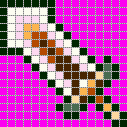
\includegraphics{video/sprite_1.png}
  \caption{Pattern Example}
\end{figure}

Using the default palette, which is initialised with RGB332 colours
from 0-255, the hexadecimal values for this pattern arranged in a
$16\times16$ array are shown below:

\begin{verbatim}
04040404040404E3E3E3E3E3E3E3E3E3
04FFFFFFFFFF04E3E3E3E3E3E3E3E3E3
04FFFBFBFBFF04E3E3E3E3E3E3E3E3E3
04FFFBF5F5FBFF04E3E3E3E3E3E3E3E3
04FFFBF5A8A8FBFF04E3E3E3E3E3E3E3
04FFFFFBA844A8FBFF04E3E3E3E3E3E3
040404FFFBA844A8FBFF04E3E3E3E3E3
E3E3E304FFFBA84444FBFF04E304E3E3
E3E3E3E304FFFB444444FBFF044D04E3
E3E3E3E3E304FFFB44444444FA4D04E3
E3E3E3E3E3E304FFFB44FFF54404E3E3
E3E3E3E3E3E3E304FF44F5A804E3E3E3
E3E3E3E3E3E3E3E304FA4404A804E3E3
E3E3E3E3E3E3E3044D4D04E304F504E3
E3E3E3E3E3E3E3E30404E3E3E304FA04
E3E3E3E3E3E3E3E3E3E3E3E3E3E30404

\end{verbatim}
Here \$E3 is used as the transparent index.

These 256 bytes would be stored in pattern memory in left to right,
top to bottom order.

\subparagraph{4-Bit Sprite Patterns}

The $16\times16$ pixel image uses 4-bits for each pixel so that each
pixel can be one of 16 colours. One colour indicates transparency and
this is programmed into the lower 4-bits of the Sprite Transparency
Index register (nextreg \$4B). By default the transparency value is
\$3. Note that the same register is shared with 8-bit patterns to
identify the transparent index.

Since each pixel only occupies 4-bits, two pixels are stored in each
byte. The leftmost pixel is stored in the upper 4-bits and the
rightmost pixel is stored in the lower 4-bits.

As an example we will use the same sprite image as was given in the
8-bit pattern example. Here only the lower 4 bits of each pixel is
retained to confine each pixel’s color to 4-bits:

\begin{verbatim}
4444444333333333
4FFFFF4333333333
4FBBBF4333333333
4FB55BF433333333
4FB588BF43333333
4FFB848BF4333333
444FB848BF433333
3334FB844BF43433
33334FB444BF4D43
333334FB4444AD43
3333334FB4F54433
33333334F4584333
333333334A448433
33333334DD434543
33333333443334A4
3333333333333344
\end{verbatim}

\$3 is used as the transparent index.

These 128 bytes would be stored in pattern memory in left to right,
top to bottom order.

The actual colour that will appear on screen will depend on the
palette, described below. The default palette will not likely generate
suitable colours for 4-bit sprites.

\subsection{Sprite Palette}
Each pixel of a sprite image is 8-bit for 8-bit patterns or 4-bit for
4-bit patterns. The pixel value is known as a pixel colour index. This
colour index is combined with the sprite’s palette offset. The palette
offset is a 4-bit value added to the top 4-bits of the pixel colour
index. The purpose of the palette offset is to allow a sprite to
change the colour of an image.

The final sprite colour index generated by the sprite hardware is then
the sum of the pixel index and the 4-bit palette offset. In pictures
using binary math:

\begin{verbatim}
8-bit Sprite
PPPP0000
+ IIIIIIII
----------
SSSSSSSS

4-bit Sprite
PPPP0000
+ 0000IIII
----------
SSSSSSSS = PPPPIIII
\end{verbatim}

Where “PPPP” is the 4-bit palette offset from the sprite’s attributes
and the “I”s represent the pixel value from the sprite pattern. The
final sprite index is represented by the 8-bit value “SSSSSSSS”.

For 4-bit sprites the palette offset can be thought of as selecting
one of 16 different 16-colour palettes.

This final 8-bit sprite index is then passed through the sprite
palette which acts like a lookup table that returns the 9-bit RGB333
colour associated with the sprite index.

At power up, the sprite palette is initialized such that the sprite
index passes through unchanged and is therefore interpretted as an
RGB332 colour. The missing third blue bit is generated as the logical
OR of the two other blue bits. In short, for 8-bit sprites, the sprite
index also acts like the colour when using the default palette.

\subsection{Sprite Attributes}
A sprite’s attributes is a list of properties that determine how and
where the sprite is drawn.

Each sprite is described by either 4 or 5 attribute bytes listed
below:

Sprite Attribute 0
\begin{verbatim}
X X X X X X X X
\end{verbatim}
The least significant eight bits of the sprite’s X coordinate. The
ninth bit is found in sprite attribute 2.

Sprite Attribute 1
\begin{verbatim}
Y Y Y Y Y Y Y Y
\end{verbatim}
The least significant eight bits of the sprite’s Y coordinate. The
ninth bit is optional and is found in attribute 4.

Sprite Attribute 2
\begin{verbatim}
P P P P XM YM R X8/PR
\end{verbatim}
P = 4-bit Palette Offset

XM = 1 to mirror the sprite image horizontally

YM = 1 to mirror the sprite image vertically

R = 1 to rotate the sprite image 90 degrees clockwise

X8 = Ninth bit of the sprite’s X coordinate

PR = 1 to indicate P is relative to the anchor’s palette offset
(relative sprites only)

Rotation is applied before mirroring.

Relative sprites, described below, replace X8 with PR.

\begin{figure}\centering
  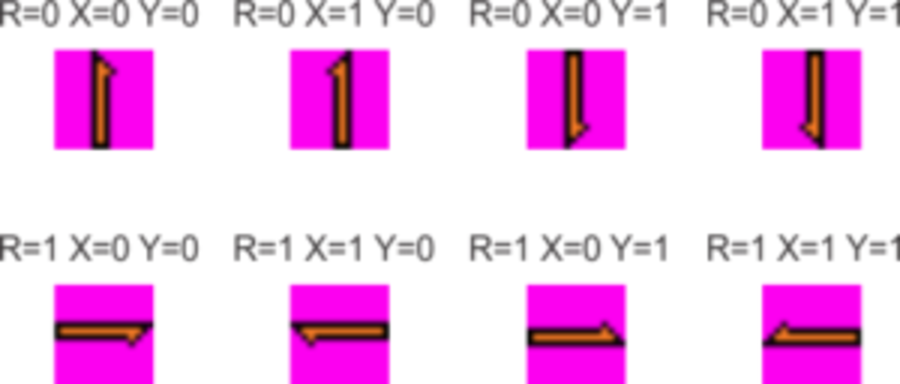
\includegraphics{video/flags.png}
  \caption{All Rotate and Mirror Flags}
\end{figure}

Sprite Attribute 3
\begin{verbatim}
V E N5 N4 N3 N2 N1 N0
\end{verbatim}
V = 1 to make the sprite visible

E = 1 to enable attribute byte 4

N = Sprite pattern to use 0-63

If E=0, the sprite is fully described by sprite attributes 0-3. The
sprite pattern is an 8-bit one identified by pattern N=0-63. The
sprite is an anchor and cannot be made relative. The sprite is
displayed as if sprite attribute 4 is zero.

If E=1, the sprite is further described by sprite attribute 4.

Sprite Attribute 4
\begin{enumerate}[A.]
\item Extended Anchor Sprite
\begin{verbatim}
H N6 T X X Y Y Y8
\end{verbatim}
H = 1 if the sprite pattern is 4-bit

N6 = 7th pattern bit if the sprite pattern is 4-bit

T = 0 if relative sprites are composite type else 1 for unified type

XX = Magnification in the X direction (00 = $1\times$, 01 = $2\times$,
10 = $4\times4$, 11 = $8\times$)

YY = Magnification in the Y direction (00 = $1\times$, 01 = $2\times$,
10 = $4\times$, 11 = $8\times$)

Y8 = Ninth bit of the sprite’s Y coordinate

{H,N6} must not equal {0,1} as this combination is used to indicate a
relative sprite.

\item Relative Sprite, Composite Type
\begin{verbatim}
0 1 N6 X X Y Y PO
\end{verbatim}
N6 = 7th pattern bit if the sprite pattern is 4-bit

XX = Magnification in the X direction (00 = $1\times$, 01 = $2\times$,
10 = $4\times$, 11 = $8\times$)

YY = Magnification in the Y direction (00 = $1\times$, 01 = $2\times$,
10 = $4\times$, 11 = $8\times$)

PO = 1 to indicate the sprite pattern number is relative to the
anchor’s

\item Relative Sprite, Unified Type
\begin{verbatim}
0 1 N6 0 0 0 0 PO
\end{verbatim}
N6 = 7th pattern bit if the sprite pattern is 4-bit

PO = 1 to indicate the sprite pattern number is relative to the
anchor’s
\end{enumerate}
The display surface for sprites is $320\times256$. The X coordinate of
the sprite is nine bits, ranging over 0-511, and the Y coordinate is
optionally nine bits again ranging over 0-511 or is eight bits ranging
over 0-255. The full extent 0-511 wraps on both axes, meaning a sprite
16 pixels wide plotted at X coordinate 511 would see its first pixel
not displayed (coordinate 511) and the following pixels displayed in
coordinates 0-14.

The full display area is visible in VGA. However, the HDMI display is
vertically shorter so the top eight pixel rows (Y = 0-7) and the
bottom eight pixel rows (Y = 248-255) will not be visible on an HDMI
display.

Sprites can be fully described by sprite attributes 0-3 if the E bit
in sprite attribute 3 is zero. These sprites are compatible with the
original sprite module from core versions prior to 2.00.26.

If the E bit is set then a fifth sprite attribute, sprite attribute 4,
becomes active. This attribute introduces scaling, 4-bit patterns, and
relative sprites. Scaling is self-explanatory and 4-bit patterns were
described in the last section. Relative sprites are described in the
next section.

\subsection{Relative Sprites}
Normal sprites (sprites that are not relative) are known as anchor
sprites. As the sprite module draws sprites in the order 0-127 (there
are 128 sprites), it internally stores characteristics of the last
anchor sprite seen. If following sprites are relative, they inherit
some of these characteristics, which allows relative sprites to have,
among other things, coordinates relative to the anchor. This means
moving the anchor sprite also causes its relatives to move with it.

There are two types of relative sprites supported known as “Composite
Sprites” and “Unified Sprites”. The type is determined by the anchor
in the T bit of sprite attribute 4.

\begin{enumerate}[A.]
\item Composite Sprites

  The sprite module records the following information from the anchor:
  \begin{itemize}
  \item Anchor.visible
  \item Anchor.Y
  \item Anchor.palette\_offset
  \item Anchor.N (pattern number)
  \item Anchor.H (indicates if the sprite uses 4-bit patterns)
  \end{itemize}
  These recorded items are not used by composite sprites:
  \begin{itemize}
  \item Anchor.rotate
  \item Anchor.xmirror
  \item Anchor.ymirror
  \item Anchor.xscale
  \item Anchor.yscale
  \end{itemize}
  The anchor determines if all its relative sprites use 4-bit patterns or not.
  
  The visibility of a particular relative sprite is the result of
  ANDing the anchor’s visibility with the relative sprite’s
  visibility. In other words, if the anchor is invisible then so are
  all its relatives.

  Relative sprites only have 8-bit X and Y coordinates (the ninth bits
  are taken for other purposes). These are signed offsets from the
  anchor’s X,Y coordinate. Moving the anchor moves all its relatives
  along with it.

  If the relative sprite has its PR bit set in sprite attribute 2,
  then the anchor’s palette offset is added to the relative sprite’s
  to determine the active palette offset for the relative
  sprite. Otherwise the relative sprite uses its own palette offset as
  usual.

  If the relative sprite has its PO bit set in sprite attribute 4,
  then the anchor’s pattern number is added to the relative sprite’s
  to determine the pattern used for display. Otherwise the relative
  sprite uses its own pattern number as usual. The intention is to
  supply a method to easily animate a large sprite by manipulating the
  pattern number in the anchor.

  A composite sprite is like a collection of independent sprites tied
  to an anchor.

\item Unified Sprites

  Unified sprites are a further extension of the
  composite type. The same information is recorded from the anchor and
  the same behaviour as described under composite sprites applies.

  The difference is the collection of anchor and relatives is treated
  as if it were a single $16\times16$ sprite. The anchor’s rotation,
  mirror, and scaling bits apply to all its relatives. Rotating the
  anchor causes all the relatives to rotate around the
  anchor. Mirroring the anchor causes the relatives to mirror around
  the anchor. The sprite hardware will automatically adjust X,Y coords
  and rotation, scaling and mirror bits of all relatives according to
  settings in the anchor.

  Unified sprites should be defined as if all its parts are
  $16\times16$ in size with the anchor controlling the look of the
  whole.

  A unified sprite is like a big version of an individual $16\times16$
  sprite controlled by the anchor.
\end{enumerate}

\subsection{Programming Sprites}

Sprites are created via three io registers and a nextreg interface.

Port \$303B (W)
\begin{verbatim}
X S S S S S S S
N6 X N N N N N N
\end{verbatim}
A write to this port has two effects.

One is it selects one of 128 sprites for writing sprite attributes via
port \$57.

The other is it selects one of 128 4-bit patterns in pattern memory
for writing sprite patterns via port \$5B. The N6 bit shown is the
least significant in the 7-bit pattern number and should always be
zero when selecting one of 64 8-bit patterns indicated by N.

Port \$57 (W)

Once a sprite is selected via port \$303B, its attributes can be
written to this port one byte after another. Sprites can have either
four or five attribute bytes and the internal attribute pointer will
move onto the next sprite after those four or five attribute bytes are
written. This means you can select a sprite via port \$303B and write
attributes for as many sequential sprites as desired. The attribute
pointer will roll over from sprite 127 to sprite 0.

Port \$5B (W)

Once a pattern number is selected via port \$303B, the 256-byte or
128-byte pattern can be written to this port. The internal pattern
pointer auto-increments after each write so as many sequential
patterns as desired can be written. The internal pattern pointer will
roll over from pattern 127 to pattern 0 (4-bit patterns) or from
pattern 63 to pattern 0 (8-bit patterns) automatically.

Port \$303B (R)

\begin{verbatim}
0 0 0 0 0 0 M C
\end{verbatim}
M = 1 if the maximum number of sprites per line was exceeded

C = 1 if any two displayed sprites collide on screen

Reading this port automatically resets the M and C bits.

Besides the i/o interface, there is a nextreg interface to sprite
attributes. The nextreg interface allows the copper to manipulate
sprites and grants the program random access to a sprite’s individual
attribute bytes.

(R/W) \$34 (52) $\Rightarrow$ Sprite Number

If the sprite number is in lockstep with io port \$303B (nextreg \$09
bit 4 is set)
\begin{itemize}
\item[] bits 7 = Pattern address offset (Add 128 to pattern address)
\item[] bits 6-0 = Sprite number 0-127, Pattern number 0-63
\end{itemize}
Selects which sprite has its attributes connected to the following registers.

Effectively performs an out to port \$303B with the same value

Otherwise
\begin{itemize}
\item[] bit 7 = Ignored
\item[] bits 6-0 = Sprite number 0-127
\end{itemize}
Selects which sprite has its attributes connected to the following registers.

Bit 7 always reads back as zero.

This nextreg can operate in two modes.

If nextreg \$09 bit 4 is set, then this register is kept in lockstep
with i/o port \$303B. A write to this nextreg is equivalent to a write
to port \$303B and vice versa. In this mode, the i/o interface and
nextreg interface are exactly equivalent.

If nextreg \$09 bit 4 is reset, then the nextreg interface is
decoupled from i/o port \$303B. This nextreg is used to select a
particular sprite 0-127 and this is completely independent from the
sprite selected for the i/o interface. This independence allows the
copper, for example, to manipulate different sprites than the cpu
using the i/o interface.

(W) \$35 (53) $\Rightarrow$ Sprite Attribute 0

(W) \$75 (117) $\Rightarrow$ Sprite Attribute 0 with automatic post
increment of Sprite Number
\begin{itemize}
\item[] bits 7-0 = LSB of X coordinate
\end{itemize}
A write to nextreg \$75 also increases the selected sprite in nextreg
\$34.

(W) \$36 (54) $\Rightarrow$ Sprite Attribute 1

(W) \$76 (118) $\Rightarrow$ Sprite Attribute 1 with automatic post
increment of Sprite Number
\begin{itemize}
\item[] bits 7-0 = LSB of Y coordinate
\end{itemize}
A write to nextreg \$76 also increases the selected sprite in nextreg
\$34.

(W) \$37 (55) $\Rightarrow$ Sprite Attribute 2

(W) \$77 (119) $\Rightarrow$ Sprite Attribute 2 with automatic post
increment of Sprite Number
\begin{itemize}
\item[] bits 7-4 = Palette offset added to top 4 bits of sprite colour
  index
\item[] bit 3 = X mirror
\item[] bit 2 = Y mirror
\item[] bit 1 = Rotate
\item[] bit 0 = MSB of X coordinate
\end{itemize}
A write to nextreg \$77 also increases the selected sprite in nextreg
\$34.

(W) \$38 (56) $\Rightarrow$ Sprite Attribute 3

(W) \$78 (120) $\Rightarrow$ Sprite Attribute 3 with automatic post
increment of Sprite Number
\begin{itemize}
\item[] bit 7 = Visible flag (1 = displayed)
\item[] bit 6 = Extended attribute (1 = Sprite Attribute 4 is active)
\item[] bits 5-0 = Pattern used by sprite (0-63)
\end{itemize}
A write to nextreg \$78 also increases the selected sprite in nextreg
\$34.

(W) \$39 (57) $\Rightarrow$ Sprite Attribute 4

(W) \$79 (121) $\Rightarrow$ Sprite Attribute 4 with automatic post
increment of Sprite Number

4-bit Sprites
\begin{itemize}
\item[] bit 7 = H (1 = sprite uses 4-bit patterns)
\item[] bit 6 = N6 (0 = use the first 128 bytes of the pattern else
  use the last 128 bytes)
\item[] bit 5 = 1 if relative sprites are composite, 0 if relative
  sprites are unified Scaling
\item[] bits 4-3 = X scaling (00 = 1x, 01 = 2x, 10 = 4x, 11 = 8x)
\item[] bits 2-1 = Y scaling (00 = 1x, 01 = 2x, 10 = 4x, 11 = 8x)
\item[] bit 0 = MSB of Y coordinate
\end{itemize}
A relative mode is enabled if H,N6 = 01. The byte format for relative
sprites is described above.

A write to nextreg \$79 also increases the selected sprite in nextreg
\$34.

\subsection{Global Control of Sprites}

The following nextreg are also of interest for sprites.

(R/W) \$09 (09) $\Rightarrow$ Peripheral 4 setting:
\begin{itemize}
\item[] bit 7 = Mono setting for AY 2 (1 = mono, 0 default)
\item[] bit 6 = Mono setting for AY 1 (1 = mono, 0 default)
\item[] bit 5 = Mono setting for AY 0 (1 = mono, 0 default)
\item[] bit 4 = Sprite id lockstep (1 = Nextreg \$34 and IO Port
  \$303B are in lockstep, 0 default)
\item[] bit 3 = Disables Kempston port (\$DF) if set
\item[] bit 2 = Disables divMMC ports (\$E3, \$E7, \$EB) if set
\item[] bits 1-0 = scanlines (0 after a PoR or Hard-reset)
  \begin{itemize}
  \item[] 00 = scanlines off
  \item[] 01 = scanlines 75\%
  \item[] 10 = scanlines 50\%
  \item[] 11 = scanlines 25\%
  \end{itemize}
\end{itemize}

Bit 4 determines if the i/o interface and nextreg interface operate in lockstep.

(R/W) \$15 (21) $\Rightarrow$ Sprite and Layers system
\begin{itemize}
\item[] bit 7 = LoRes mode, $128\times96\times256$ colours (1 =
  enabled)
\item[] bit 6 = Sprite priority (1 = sprite 0 on top, 0 = sprite 127
  on top)
\item[] bit 5 = Enable sprite clipping in over border mode (1 =
  enabled)
\item[] bits 4-2 = set layers priorities:

Reset default is 000, sprites over the Layer 2, over the ULA graphics
\begin{itemize}
\item[] 000 – S L U
\item[] 001 – L S U
\item[] 010 – S U L
\item[] 011 – L U S
\item[] 100 – U S L
\item[] 101 – U L S
\item[] 110 – S(U+L) ULA and Layer 2 combined, colours clamped to 7
\item[] 111 – S(U+L-5) ULA and Layer 2 combined, colours clamped to
  [0,7]
\end{itemize}
\item[] bit 1 = Over border (1 = yes)(Back to 0 after a reset)
\item[] bit 0 = Sprites visible (1 = visible)(Back to 0 after a reset)
\end{itemize}

Bit 0 must be set for sprites to be visible.

Bit 1 set allows sprites to be visible in the border area. When this
bit is reset, sprites will not display outside the $256\times192$ area
of the ULA display.

Bit 5 set enables clipping when sprites are visible in the border
area. If reset, no clipping is applied and sprites will be visible in
the full $320\times256$ space.

The sprite module draws sprites in the order 0-127 in each
scanline. Bit 6 determines whether sprite 0 is topmost or sprite 127
is topmost.

Bits 4:2 determine layer priority and how sprites overlay or are
obscured by other layers.

(R/W) \$19 (25) $\Rightarrow$ Clip Window Sprites
\begin{itemize}
\item[] bits 7-0 = Cood. of the clip window
  \begin{itemize}
  \item[] 1st write – X1 position
  \item[] 2nd write – X2 position
  \item[] 3rd write – Y1 position
  \item[] 4rd write – Y2 position
  \end{itemize}
\end{itemize}
The values are 0,255,0,191 after a Reset

Reads do not advance the clip position

When the clip window is enabled for sprites in “over border” mode, the
X coords are internally doubled and the clip window origin is moved to
the sprite origin inside the border.

Sprites will only be visible inside the clipping window. When not in
over-border mode (bit 1 of nextreg \$15) the clipping window is given
in ULA screen coordinates with 0,0 correspoding to the top left corner
of the ULA screen. In over-border mode, the clipping window’s origin
is moved to the sprite coordinate origin 32 pixels to the left and 32
pixels above the ULA screen origin.

Regardless, sprite position is always in sprite coordinates with 32,32
corresponding to the top left corner of the ULA screen.

(W) \$1C (28) $\Rightarrow$ Clip Window control
\begin{itemize}
\item[] bits 7-4 = Reserved, must be 0
\item[] bit 3 – reset the tilemap clip index
\item[] bit 2 – reset the ULA/LoRes clip index.
\item[] bit 1 – reset the sprite clip index.
\item[] bit 0 – reset the Layer 2 clip index.
\end{itemize}

Can be used to reset nextreg \$19.

(R/W) \$43 (67) $\Rightarrow$ Palette Control
\begin{itemize}
\item[] bit 7 = ‘1’ to disable palette write auto-increment.
\item[] bits 6-4 = Select palette for reading or writing:
  \begin{itemize}
  \item[] 000 = ULA first palette
  \item[] 100 = ULA second palette
  \item[] 001 = Layer 2 first palette
  \item[] 101 = Layer 2 second palette
  \item[] 010 = Sprites first palette
  \item[] 110 = Sprites second palette
  \item[] 011 = Tilemap first palette
  \item[] 111 = Tilemap second palette
  \end{itemize}
\item[] bit 3 = Select Sprites palette (0 = first palette, 1 = second
  palette)
\item[] bit 2 = Select Layer 2 palette (0 = first palette, 1 = second
  palette)
\item[] bit 1 = Select ULA palette (0 = first palette, 1 = second
  palette)
\item[] bit 0 = Enabe ULANext mode if 1. (0 after a reset)
\end{itemize}

Sprites have two associated palettes which can be selected in this nextreg.

(R/W) \$40 (64) $\Rightarrow$ Palette Index
\begin{itemize}
\item[] bits 7-0 = Select the palette index to change the associated
  colour.
\end{itemize}
For the ULA only, INKs are mapped to indices 0-7, Bright INKS to
indices 8-15, PAPERs to indices 16-23 and Bright PAPERs to indices
24-31.

In ULANext mode, INKs come from a subset of indices 0-127 and PAPERs
come from a subset of indices 128-255. The number of active indices
depends on the number of attribute bits assigned to INK and PAPER out
of the attribute byte.  The ULA always takes border colour from paper.

Select the starting palette index if writing the sprite palette.

Palette values can be written in either 8-bit or 9-bit form:

(R/W) \$41 (65) $\Rightarrow$ Palette Value (8 bit colour)
\begin{itemize}
\item[] bits 7-0 = Colour for the palette index selected by the register \$40.
\end{itemize}
(Format is RRRGGGBB – the lower blue bit of the 9-bit colour will be a
logical OR of blue bits 1 and 0 of this 8-bit value.)

After the write, the palette index is auto-incremented to the next
index if the auto-increment is enabled at reg \$43. Reads do not
auto-increment.

(R/W) \$44 (68) $\Rightarrow$ Palette Value (9 bit colour)

Two consecutive writes are needed to write the 9 bit colour
\begin{itemize}
\item[] 1st write:
  \begin{itemize}
  \item[] bits 7-0 = RRRGGGBB
  \end{itemize}
\item[] 2nd write.
  If writing a L2 palette
  \begin{itemize}
  \item[] bit 7 = 1 for L2 priority colour, 0 for normal

    Priority colour will always be on top even on an SLU priority
    arrangement. If you need the exact same colour on priority and non
    priority locations you will need to program the same colour twice
    changing bit 7 to 0 for the second colour
  \item[] bits 6-1 = Reserved, must be 0
  \item[] bit 0 = lsb B
  \end{itemize}
  
  If writing another palette
  \begin{itemize}
  \item[] bits 7-1 = Reserved, must be 0
  \item[] bit 0 = lsb B
  \end{itemize}
\end{itemize}


After the two consecutives writes the palette index is
auto-incremented if the auto-increment is enabled by reg \$43.

Reads only return the 2nd byte and do not auto-increment.

(R/W) \$4B (75) $\Rightarrow$ Transparency index for sprites
\begin{itemize}
\item[] bits 7-0 = Set the index value (\$E3 after reset)
\end{itemize}
For 4-bit sprites only the bottom 4-bits are relevant.

Determines the transparent colour index used for sprites.

\end{multicols}
